\documentclass{beamer}

\usepackage[utf8]{inputenc}
\usetheme{Copenhagen}
\usepackage{amssymb}
\usepackage{pifont}
\usepackage{tikz}
\usetikzlibrary{automata, positioning, arrows}



\newcommand{\xmark}{\ding{55}}%
\newcommand{\cmark}{\ding{51}}


\title[Robot Motion Planning]{Robot Motion Planning}
\author{F. Barbosa, K. Grover, J. K\v{r}et\'{i}nsk\'{y}, J. Tumova}
%\author{Presented by Kush}
\date{}
\begin{document}
	\frame{\titlepage}
	
	\begin{frame}
		\frametitle{Motion Planning Problem}
		\begin{center}
			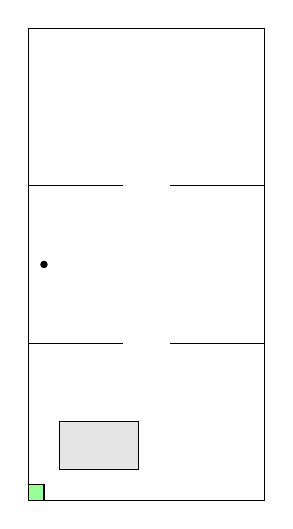
\begin{tikzpicture}
				\filldraw[fill = green!40!white, draw = black] (0, 0) rectangle (0.2, 0.2);
				\filldraw[fill = black!10!white, draw = black] (0.4, 0.4) rectangle (1.4, 1);
				\draw (0, 0) -- (3, 0) -- (3, 6) -- (0, 6) -- (0, 0);
				\draw (0, 2) -- (1.2, 2) (1.8, 2) -- (3, 2);
				\draw (0, 4) -- (1.2, 4) (1.8, 4) -- (3, 4);
				\filldraw[black] (0.2, 3) circle (0.4mm);
			\end{tikzpicture}
		\end{center}
	\end{frame}
	
	\begin{frame}
		\frametitle{RRG}
		\begin{center}
			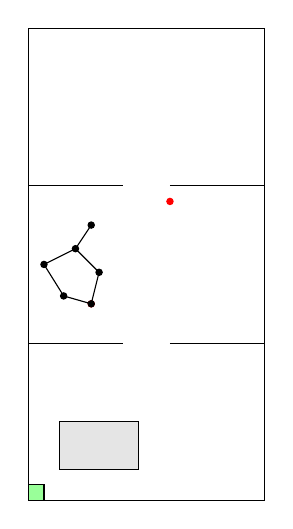
\begin{tikzpicture}
			\onslide<0->{
				\filldraw[fill = green!40!white, draw = black] (0, 0) rectangle (0.2, 0.2);
				\filldraw[fill = black!10!white, draw = black] (0.4, 0.4) rectangle (1.4, 1);
				\draw (0, 0) -- (3, 0) -- (3, 6) -- (0, 6) -- (0, 0);
				\draw (0, 2) -- (1.2, 2) (1.8, 2) -- (3, 2);
				\draw (0, 4) -- (1.2, 4) (1.8, 4) -- (3, 4);
				\filldraw[black] (0.2, 3) circle (0.4mm);
			}
			\onslide<1-2>{
				\filldraw[red] (1.8, 3.8) circle (0.4mm);
			}
			\onslide<2->{
				\filldraw[black] (0.6, 3.2) circle (0.4mm);
				\draw (0.2,3) -- (0.6, 3.2);
			}
			\onslide<3->{
				\filldraw[black] (0.45, 2.6) circle (0.4mm);
				\draw (0.2,3) -- (0.45, 2.6);
				\filldraw[black] (0.8, 3.5) circle (0.4mm);
				\draw (0.6,3.2) -- (0.8, 3.5);
				\filldraw[black] (0.9, 2.9) circle (0.4mm);
				\draw (0.6,3.2) -- (0.9, 2.9);
			}
			\onslide<4>{
				\filldraw[red] (0.8, 2.5) circle (0.4mm);
			}
			\onslide<5->{
				\filldraw[black] (0.8, 2.5) circle (0.4mm);
				\draw (0.45, 2.6) -- (0.8, 2.5);
				\draw (0.9, 2.9) -- (0.8, 2.5);
			}
			\end{tikzpicture}
		\end{center}
	\end{frame}

	\begin{frame}
		\frametitle{Jan's vision}
		\begin{itemize}
		\item Want a robot that can move around on its own and figure out the stuff it has to do. \pause \textcolor{red}{\xmark}\\
		Too big a goal right now from both theoretical and practical perspectives.\\
		\pause \vspace{10pt}
		What can we do?\\
		Reachability. \textcolor{green}{\cmark} \pause\\
		LTL or a subclass of LTL. \\
		Given a labeling of the environment. Find a path that satisfies a given LTL formula.
		\end{itemize}
	\end{frame}


	\begin{frame}
		\frametitle{LTL Motion Planning}
		\begin{center}
			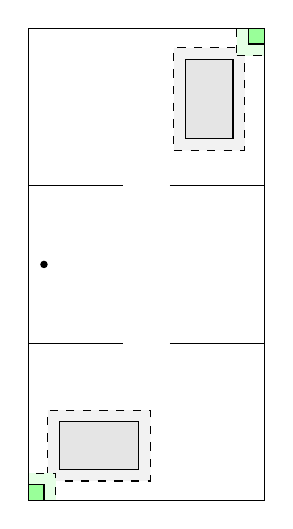
\begin{tikzpicture}
			\filldraw[dashed, fill = gray!10!white] (0.25,0.25) -- (1.55,0.25) -- (1.55,1.15) -- (0.25,1.15) -- (0.25, 0.25);
			\filldraw[dashed, fill = green!10!white] (0,0) -- (0.35,0) -- (0.35,0.35) -- (0,0.35) -- (0,0);
			\filldraw[dashed, fill = gray!10!white] (1.85,4.45) -- (2.75,4.45) -- (2.75,5.75) -- (1.85,5.75) -- (1.85, 4.45);
			\filldraw[dashed, fill = green!10!white] (2.65,5.65) -- (3,5.65) -- (3,6) -- (2.65,6) -- (2.65,5.65);
			
			\filldraw[fill = green!40!white, draw = black] (0, 0) rectangle (0.2, 0.2);
			\filldraw[fill = black!10!white, draw = black] (0.4, 0.4) rectangle (1.4, 1);
			\filldraw[fill = green!40!white, draw = black] (2.8, 5.8) rectangle (3, 6);
			\filldraw[fill = black!10!white, draw = black] (2, 4.6) rectangle (2.6, 5.6);
			
			\draw (0, 0) -- (3, 0) -- (3, 6) -- (0, 6) -- (0, 0);
			\draw (0, 2) -- (1.2, 2) (1.8, 2) -- (3, 2);
			\draw (0, 4) -- (1.2, 4) (1.8, 4) -- (3, 4);
			\filldraw[black] (0.2, 3) circle (0.4mm);
			\end{tikzpicture}
			
			\emph{Specification:} $G F (r_1 \wedge b) \wedge G F (r_2 \wedge b)$
		\end{center}
	\end{frame}

	\begin{frame}
		\frametitle{Solution}
		\begin{itemize}
			\item Build an abstraction of the system.
			\item Construct the product automaton with the property automaton (ldba).
			\item Find a path in the abstraction.
			\item Lift this path to the original system.
		\end{itemize}
	\end{frame}
	
	\begin{frame}
		\frametitle{Better Solution}
		Can we do better?\\ \pause \vspace{10pt}
		\textbf{Jan's idea:} Get help in sampling from current abstraction. \\
		Depending on previous experiences. In other words, predict which samples would be better from previous samples. \\ \pause \vspace{10pt}
		For e.g: The bin was close to the table in first room so try to look close to the table in the other room to find the bin.
	\end{frame}

	\begin{frame}
		\frametitle{Better Solution}
		How do we formalize this? \\ \pause
		\begin{itemize}
			\item Have `maybe' and `maybe not' transitions in the abstraction.\\
			\item Whenever you see a transition, add similar `maybe' transitions in the abstraction as well.
			\item What does similar mean here?\\
			$(r_1, t) \rightarrow (r_1, b) \implies (r_2, t) \rightarrow (r_2,b)$. \\
			\begin{itemize}
				\item Compute domain of changes: Set of APs changing in a transition.\\
				$DOC = \{t,b\}$, $(s_1 \oplus s_2)$
				\item Add transitions $s_1' \rightarrow s_2'$ where $s_1'$ and $s_2'$ are states which agree with $s_1$ and $s_2$ on $DOC$ respectively.
			\end{itemize}
		\end{itemize}
	\end{frame}
	
	\begin{frame}
		\frametitle{Algorithm}
		\begin{center}
			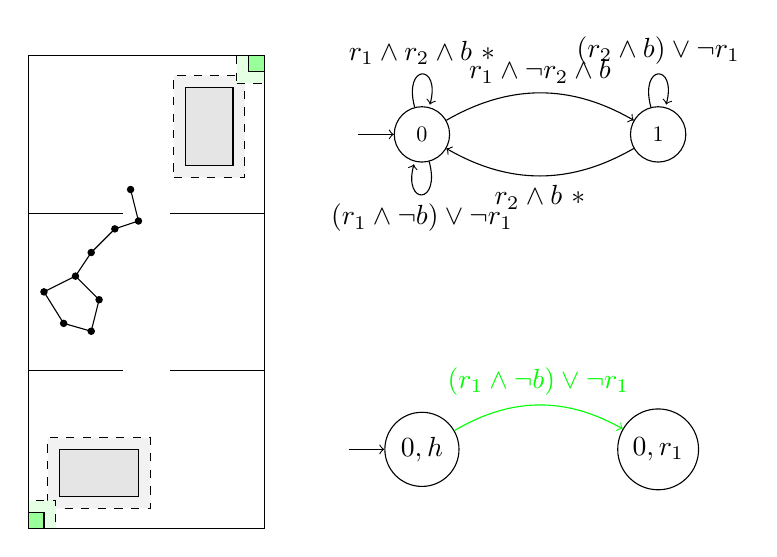
\begin{tikzpicture}
			\filldraw[dashed, fill = gray!10!white] (0.25,0.25) -- (1.55,0.25) -- (1.55,1.15) -- (0.25,1.15) -- (0.25, 0.25);
			\filldraw[dashed, fill = green!10!white] (0,0) -- (0.35,0) -- (0.35,0.35) -- (0,0.35) -- (0,0);
			\filldraw[dashed, fill = gray!10!white] (1.85,4.45) -- (2.75,4.45) -- (2.75,5.75) -- (1.85,5.75) -- (1.85, 4.45);
			\filldraw[dashed, fill = green!10!white] (2.65,5.65) -- (3,5.65) -- (3,6) -- (2.65,6) -- (2.65,5.65);
			
			\filldraw[fill = green!40!white, draw = black] (0, 0) rectangle (0.2, 0.2);
			\filldraw[fill = black!10!white, draw = black] (0.4, 0.4) rectangle (1.4, 1);
			\filldraw[fill = green!40!white, draw = black] (2.8, 5.8) rectangle (3, 6);
			\filldraw[fill = black!10!white, draw = black] (2, 4.6) rectangle (2.6, 5.6);
			
			\draw (0, 0) -- (3, 0) -- (3, 6) -- (0, 6) -- (0, 0);
			\draw (0, 2) -- (1.2, 2) (1.8, 2) -- (3, 2);
			\draw (0, 4) -- (1.2, 4) (1.8, 4) -- (3, 4);
			\filldraw[black] (0.2, 3) circle (0.4mm);
			
			\onslide<2->{
				\node[state,initial,initial text=,scale=0.8] (q1) at (5,5) {$0$};
				\node[state,scale=0.8] (q2) at (8,5) {$1$};
				
				\draw (q1) edge[loop above] node{$r_1 \wedge r_2 \wedge b\ \ast$} (q1);
				\draw (q1) edge[loop below] node{$(r_1 \wedge \neg b) \vee \neg r_1$} (q1);
				\draw (q1) edge[bend left, above, ->] node{$r_1 \wedge \neg r_2 \wedge b$} (q2);
				\draw (q2) edge[loop above] node{$(r_2 \wedge b) \vee \neg r_1$} (q2);
				\draw (q2) edge[bend left, below, ->] node{$r_2 \wedge b\ \ast$} (q1);
			}
		
			\onslide<2->{
				\filldraw[black] (0.6, 3.2) circle (0.4mm);
				\draw (0.2,3) -- (0.6, 3.2);
				\filldraw[black] (0.45, 2.6) circle (0.4mm);
				\draw (0.2,3) -- (0.45, 2.6);
				\filldraw[black] (0.8, 3.5) circle (0.4mm);
				\draw (0.6,3.2) -- (0.8, 3.5);
				\filldraw[black] (0.9, 2.9) circle (0.4mm);
				\draw (0.6,3.2) -- (0.9, 2.9);
				\filldraw[black] (0.8, 2.5) circle (0.4mm);
				\draw (0.45, 2.6) -- (0.8, 2.5);
				\draw (0.9, 2.9) -- (0.8, 2.5);
				\filldraw[black] (1.1, 3.8) circle (0.4mm);
				\draw (0.8, 3.5) -- (1.1, 3.8);
				\filldraw[black] (1.4, 3.9) circle (0.4mm);
				\draw (1.1, 3.8) -- (1.4, 3.9);
			}
			
			\onslide<3->{
				\filldraw[black] (1.3, 4.3) circle (0.4mm);
				\draw (1.4, 3.9) -- (1.3, 4.3);
				
				\node[state,initial,initial text=] (0h) at (5,1) {$0,h$};
			}
			\onslide<4->{
				\node[state] (0r1) at (8,1) {$0,r_1$};
				\draw (0h) edge[color = green, bend left, above, ->] node{$(r_1 \wedge \neg b) \vee \neg r_1$} (0r1);
			}
			\end{tikzpicture}
		\end{center}
	\end{frame}


	\begin{frame}
		\frametitle{Learn}
		\begin{itemize}
			\item Sample a transition $s_1$ to $s_2$. 	\pause
			\item Add similar transitions.	\pause
			\item If $s_1$ has been visited 50 times, all the `maybe' transitions gets converted to `maybe not' transitions.
		\end{itemize}
	\end{frame}

	\begin{frame}
		\frametitle{Ask}
			\begin{itemize}
				\item Maintain a set of states in the abstraction which we have visited till now, \emph{visitedStates}. \pause
				\item Look at the accepting `maybe' transitions and get a list of sets of states $reach[n]$, such that $reach[i]$ will have all the states in \emph{visitedStates} that can reach an accepting transition in $i$ steps. First try to sample transitions from $reach[1] \rightarrow reach[0]$, then from $reach[2] \rightarrow reach[1]$ and so on.
			\end{itemize}
			
	\end{frame}

	\begin{frame}
		\frametitle{What's next?}
		\begin{itemize}
			\item `Definitely not' transitions. \pause
			\item Can we do full LTL? or LTL $\setminus \{X\}$. \pause
			\item What kind of filters can we use to learn useful similar transitions? \pause
			\item Make implementation faster. \pause
			\item Figure out the best thresholds. 	\pause
			\item Still very hard because we have to compete with very efficient algorithm.
		\end{itemize}
		
	\end{frame}


	\begin{frame}
		\frametitle{After this project}
		\begin{itemize}
			\item A robot that does not have information of the whole environment and can only look at things nearby. \pause
			\item Figure out atomic propositions as it goes on to make learning better (not the ones in the property).
		\end{itemize}
	\end{frame}
	
	
\end{document}